%% Latex Template for 16-720J student reports
%% You should maintain the template format wherever practical
%% Gary Overett 2015

\documentclass[12pt]{article}
\usepackage{amsmath}
\usepackage{amssymb}
\usepackage{amsthm}
\usepackage{amscd}
\usepackage{amsfonts}
\usepackage{graphicx}%
\usepackage{subcaption}
\usepackage{fancyhdr}
\usepackage{tablefootnote}
\usepackage{subcaption}
\usepackage[table]{xcolor}
\usepackage{array,multirow}
\usepackage{hyperref}
\usepackage{enumerate}
\usepackage{bm}
\usepackage{relsize}
\usepackage{titling}
\usepackage{titlesec}
\usepackage[a4paper, margin=2cm]{geometry}

\usepackage[framed, numbered, autolinebreaks, useliterate]{mcode}

\titleformat{\subsubsection}[runin]{\bf}{Question \arabic{section}.\arabic{subsection}.\arabic{subsubsection} }{0pt}{}[]
\renewcommand{\thesubsection}{\bf Question \arabic{section}.\arabic{subsection}}

\newcounter{list}

\newcommand{\fixme}{{\color{pink}FIXME!!!}}

\setlength{\droptitle}{-2cm} % less room above the title

\begin{document}


\title{16-720J: Homework 5\\RANSAC and 3D Reconstruction}

\author{Wenbo Zhao}

\maketitle

\vspace{-1cm}

\section{Theory Questions}

\subsection{(5pts)}
Assume one correspondence on the images is $p_1$, $p_2$. After normalization $\hat{p}_1 = [0,0,1]^T$, $\hat{p}_2 = [0,0,1]^T$. We have 
$$\hat{p}_1^T F \hat{p}_2=0,$$ yields
$$[0\, 0\, 1] \left [\begin{matrix} F_{1,1}\, F_{1,2}\, F_{1,3}\\ F_{2,1}\, F_{2,2}\, F_{2,3}\\ F_{3,1}\, F_{3,2}\, F_{3,3} \end{matrix} \right ][0\, 0\, 1]^T = F_{3,3} = 0$$

\subsection{(10 pts)}
\label{q:1.2}

Fundamental matrix $F=K^{-T}EK'^{-1}=K^{-T}[t]_{\times}RK'^{-1}$.
When two cameras differ only from pure translation with $x$ axis, we have
$$K=K'\,\,\,R=I$$($I$ is identity matrix)
$$t=[1\, 0\, 0]^T$$ (suppose translation is $1$)
thus yields
$$F=[t]_{\times}=\left [\begin{matrix} 0\,\,\, 0\,\,\, 0 \\ 0\,\,\, 0\, -1 \\ 0\,\,\, 1\,\,\, 0\end{matrix}\right ]$$
such follows for $p=[x\, y\, 1]^T$ and $p'=[x'\, y'\, 1]^\tau$
$$p'^TFp = 0\,\,\,\,y=y'$$
which means epipolar lines are parallel to $x$ axis.
\subsection{(10 pts)}
When viewing the image of an object and its image in the mirror, the correspondences in the two images differ only with inversed depth, \emph{i.e.} $p = [x\, y\, z]$ and $p'=[x\,y\,-z]$. This is equivalent to two cameras viewing the object in the mirror plane, and the two cameras differ from each other with pure translation parallel to depth axis. Such we have proved in \ref{q:1.2} that in this case $F$ is skew-symmetric ($x^TFx=0$ for any $x$).

\subsection{(10 pts)}
(1)Given $p_1$ and $H$, we have
$$p_2 = Hp_1$$
the epipolar line is
$$l = [e_2]_{\times}p_2 = [e_2]_{\times}Hp_1$$
(2)
NO. Because when pure translation $t=[ 0\, 0\, 0 ]^T$,
$$F=K^{-T}EK'^{-1}=K^{-T}[t]_{\times}RK'^{-1} = 0,$$
then $l=Fp_2=0$, not work.
\section{Implementation Questions}

\paragraph{\Large{Fundamental matrix estimation}}

\paragraph{The Eight Point Algorithm\\}

\subsection{(10 pts)}
$F_{8,clean}=$
\begin{verbatim}
   -0.0000    0.0000   -0.0003
   -0.0000   -0.0000    0.0021
    0.0001   -0.0022    0.1811
\end{verbatim}
$F_{8,noisy}=$
\begin{verbatim}
   -0.0000   -0.0000    0.0002
   -0.0000    0.0000    0.0017
    0.0001   -0.0019    0.0016
\end{verbatim}
$F_{8,clean}$ is more accurate because it is more close to skew-symmetric matrix.

\begin{figure}[htbp]
\begin{minipage}{\linewidth}
\centering 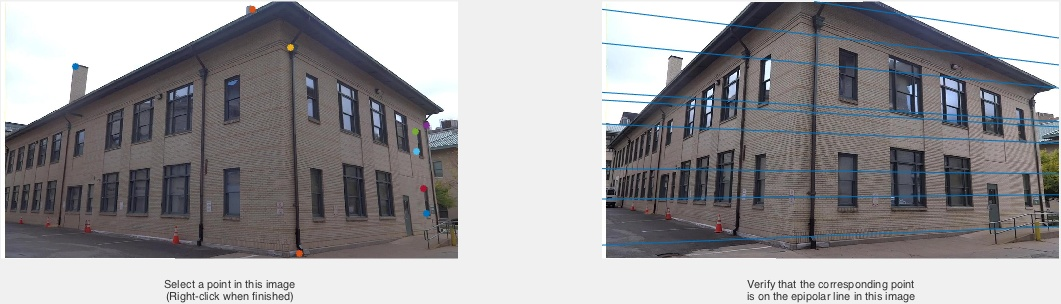
\includegraphics[width=6in]{../matlab/displayEpipolarF_clean.jpg}
\caption*{clean}
\end{minipage}
\begin{minipage}{\linewidth}
\centering 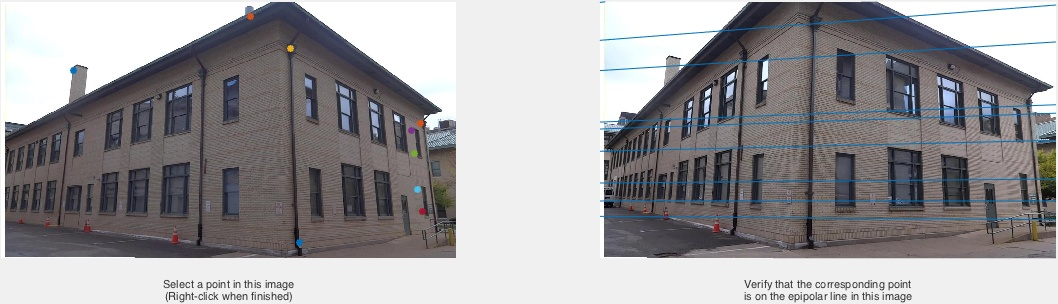
\includegraphics[width=6in]{../matlab/displayEpipolarF_noisy.jpg}
\caption*{noisy}
\end{minipage}
\caption{Display epipolar.}
\end{figure}

\lstinputlisting{../matlab/eightpoint_norm.m}

\paragraph{The Seven Point Algorithm}

\subsection{(15 pts)}
$F_{7,clean}=$
\begin{verbatim}
    0.0000   -0.0000    0.0052
    0.0000    0.0000   -0.0473
   -0.0023    0.0488    1.0698
\end{verbatim}

\begin{figure}[htbp]
\centering 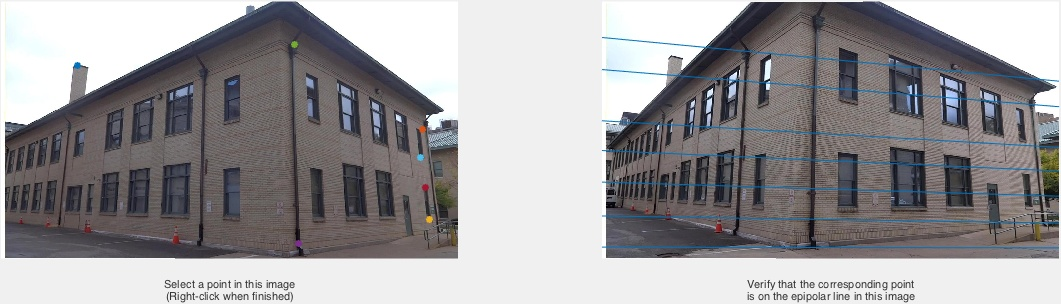
\includegraphics[width=6in]{../matlab/displayEpipolarF_clean_7point.jpg}
\caption{Display epipolar: clean, seven point.}
\end{figure}

\lstinputlisting{../matlab/sevenpoint_norm.m}

\paragraph{Computing $F$ from Noisy Correspondences with RANSAC}

\subsection{(10 pts)}
$F_{7,ransac}=$
\begin{verbatim}
    0.0000    0.0000   -0.0002
   -0.0000   -0.0000    0.0017
   -0.0000   -0.0019    0.3012
\end{verbatim}

\begin{figure}[htbp]
\centering 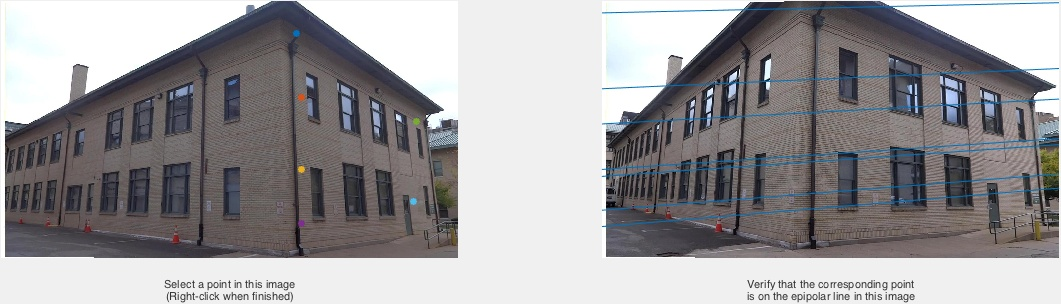
\includegraphics[width=6in]{../matlab/displayEpipolarF_noisy_7point_ransac}
\caption{Display epipolar: noisy, ransac.}
\end{figure}

\lstinputlisting{../matlab/ransacF.m}

\paragraph{Generating Novel Views of Smith Hall}

\subsection{(30 pts)}
$F_{7,ransac}=$
\begin{verbatim}
   -0.0000   -0.0000    0.0004
   -0.0000    0.0000    0.0065
   -0.0000   -0.0065    0.3715
\end{verbatim}
\begin{verbatim}
smith_south_plane =

   -0.3110
   -0.0956
   -0.2955
    0.8982
\end{verbatim}
\begin{verbatim}
smith_south_plane =

   -0.3110
   -0.0956
   -0.2955
    0.8982
\end{verbatim}

\begin{figure}[htbp]
\begin{minipage}{0.5\linewidth}
\centering 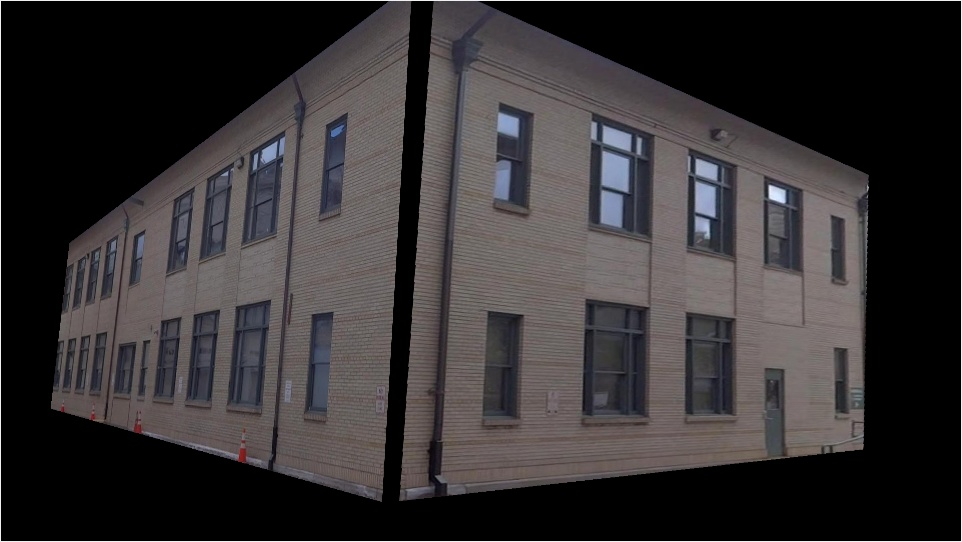
\includegraphics[width=3in]{../matlab/novel_view_1.jpg}
\caption*{novel view 1}
\end{minipage}
\begin{minipage}{0.5\linewidth}
\centering 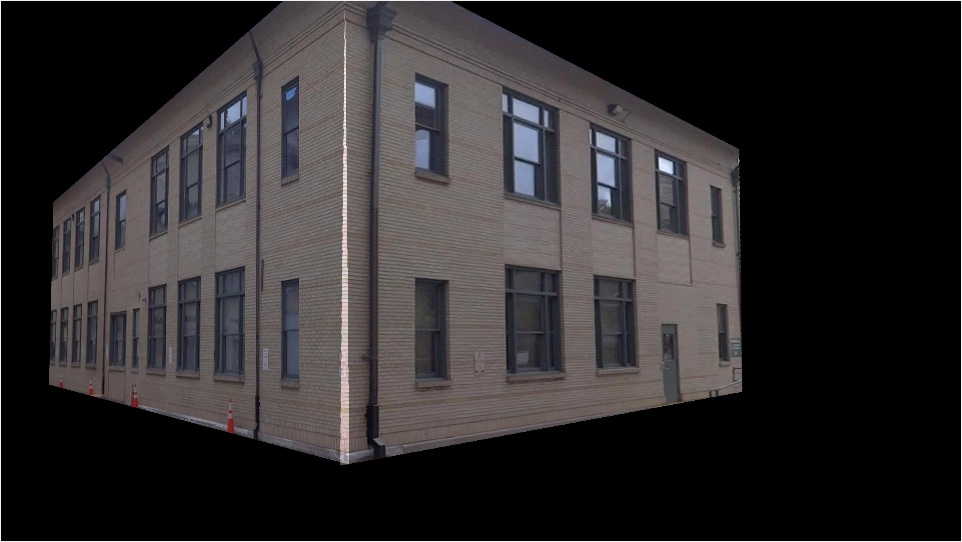
\includegraphics[width=3in]{../matlab/novel_view_2.jpg}
\caption*{novel view 2}
\end{minipage}
\begin{minipage}{0.5\linewidth}
\centering 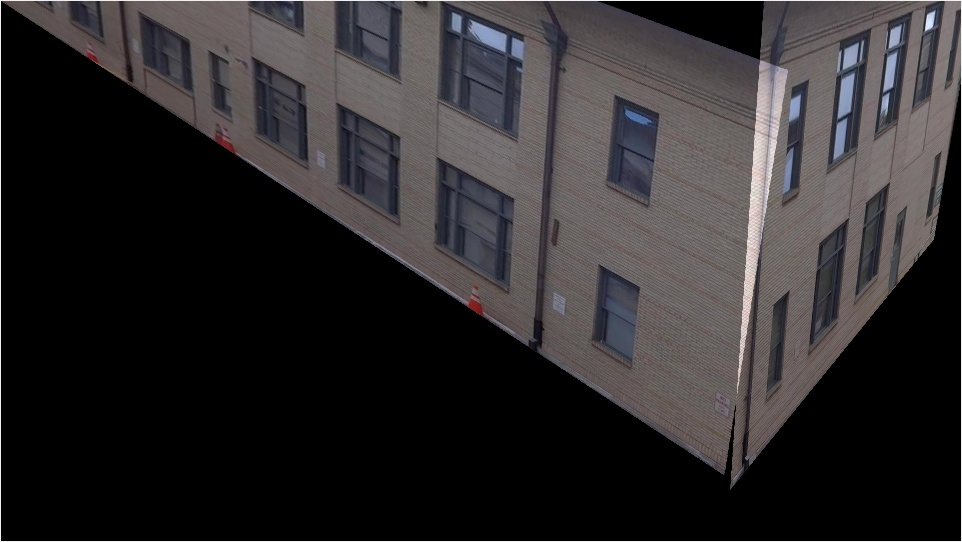
\includegraphics[width=3in]{../matlab/novel_view_3.jpg}
\caption*{novel view 3}
\end{minipage}
\begin{minipage}{0.5\linewidth}
\centering 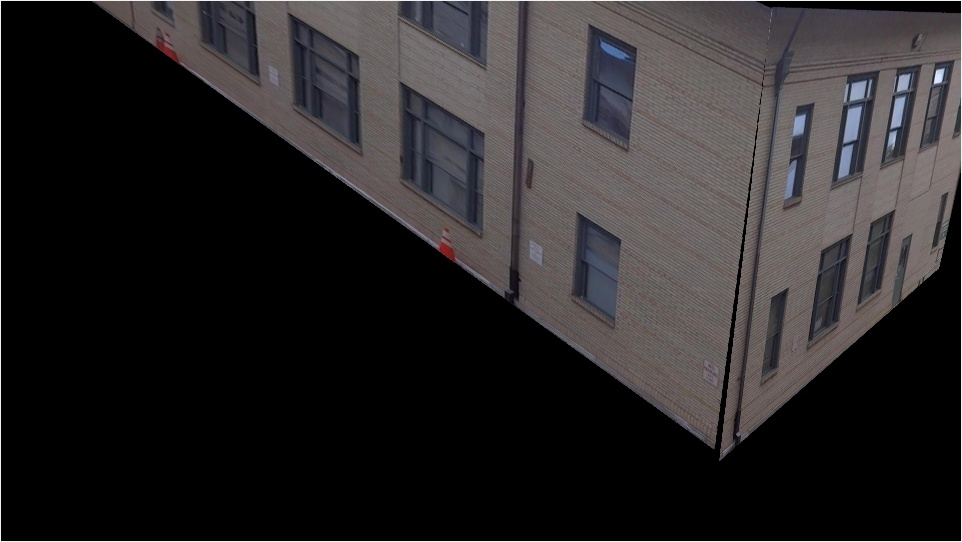
\includegraphics[width=3in]{../matlab/novel_view_4.jpg}
\caption*{novel view 4}
\end{minipage}
\caption{Novel views of Smith Hall}
\end{figure}

\begin{enumerate}[(1)]
\item Find fundamental matrix with RANSAC using seven point algorithm.
\item Generate camera matrix $M_1$ and $M_2$, and then compute the spatial point $P$ with triangulation.
\item Use RANSAC again to fit a plane model and the inliers that belong to this plane, then use the rest points to find another plane.
\item Draw the novel view.
\end{enumerate}

\lstinputlisting{../matlab/genNovelView.m}
\lstinputlisting{../matlab/ransacP.m}
\end{document}
